%% LaTeX template for BSc Computing for Games final year project dissertations
%% by Edward Powley
%% Games Academy, Falmouth University, UK

%% Based on:
%% bare_jrnl.tex
%% V1.4b
%% 2015/08/26
%% by Michael Shell
%% see http://www.michaelshell.org/
%% for current contact information.
%%
%% This is a skeleton file demonstrating the use of IEEEtran.cls
%% (requires IEEEtran.cls version 1.8b or later) with an IEEE
%% journal paper.
%%
%% Support sites:
%% http://www.michaelshell.org/tex/ieeetran/
%% http://www.ctan.org/pkg/ieeetran
%% and
%% http://www.ieee.org/

%%*************************************************************************
%% Legal Notice:
%% This code is offered as-is without any warranty either expressed or
%% implied; without even the implied warranty of MERCHANTABILITY or
%% FITNESS FOR A PARTICULAR PURPOSE! 
%% User assumes all risk.
%% In no event shall the IEEE or any contributor to this code be liable for
%% any damages or losses, including, but not limited to, incidental,
%% consequential, or any other damages, resulting from the use or misuse
%% of any information contained here.
%%
%% All comments are the opinions of their respective authors and are not
%% necessarily endorsed by the IEEE.
%%
%% This work is distributed under the LaTeX Project Public License (LPPL)
%% ( http://www.latex-project.org/ ) version 1.3, and may be freely used,
%% distributed and modified. A copy of the LPPL, version 1.3, is included
%% in the base LaTeX documentation of all distributions of LaTeX released
%% 2003/12/01 or later.
%% Retain all contribution notices and credits.
%% ** Modified files should be clearly indicated as such, including  **
%% ** renaming them and changing author support contact information. **
%%*************************************************************************


\documentclass[journal]{IEEEtran}

\usepackage{graphicx}
% Insert additional usepackage commands here
\usepackage{amsmath}
\usepackage{wrapfig}
\graphicspath{ {./images/} }


\begin{document}
%
% paper title
% Titles are generally capitalized except for words such as a, an, and, as,
% at, but, by, for, in, nor, of, on, or, the, to and up, which are usually
% not capitalized unless they are the first or last word of the title.
% Linebreaks \\ can be used within to get better formatting as desired.
% Do not put math or special symbols in the title.
\title{Comparing game tree search techniques for general video game artificial intelligence (GVGAI)}
%
%
% author name
\author{Alastair Rayner - 1507516}

% The paper headers -- please do not change these, but uncomment one of them as appropriate
% Uncomment this one for COMP320
\markboth{COMP320: Research Review and Proposal}{COMP320: Research Review and Proposal}
% Uncomment this one for COMP360
% \markboth{COMP360: Dissertation}{COMP360: Dissertation}

% make the title area
\maketitle

% As a general rule, do not put math, special symbols or citations
% in the abstract or keywords.
\begin{abstract}
The abstract goes here.
\end{abstract}

\section{Introduction}
\IEEEPARstart{T}{his} Literature review will cover what questions I will be asking for my dissertation topic as well all the literature I have found that is related to my research questions.


%NOTES

% Cite original papers, i.e. MCTS and minimax ect.
% Fix renferences
% Go into depth on the different controllers
% Go into depth on the different search tecniques
% Check for spelling
% Compare and contrast papers
% Redo hypothesis
%types of games in gvgai
%compare and contrast ALE vs GVGAI


\section{Research Questions}

%TODO: Simplify research questions
\begin{itemize}
    \item How does game tree search techniques compare for GVGAI? 
    \item Where does each tree search technique do well in each game? 
    \item What are the strengths and weaknesses of different search techniques and how can they be improved? 
\end{itemize}

\section{Hypothesis}
In progress (will deffo change) \par
Does tree search algorithms perform better than Evolutionary Algorithms?
Where does tree search algorithms out perform Evolutionary Algorithms?

\section{Literature Review}

	\subsection{General Artificial Intelligence in games}
		Games play an important role in the development and bench-marking of Artificial Intelligence (AI). This literature review will cover the existing work around the general video game artificial intelligence competition and the different solutions that are available.
		There have been a lot of popular games that have been used to benchmark AI, for example games such as chess, or Go. Some of these AI programs have been improved upon until they can defeat the world champion players, such as Deep Blue which defeated Gary Kasparov in 1997 \cite{DeepBlue, shannon1988programming, DeepBlueOverview}. 
		
		A long standing goal of AI is to develop algorithms capable of completing various tasks without any need to create domain specific tailoring.
		%Programming Chess
		Deep blue was developed at IBM during the mid-1990s. It was able to beat the world chess champion by having a massively parallel system that was able to search a very large search space concurrently \cite{DeepBlue}.

		%Programming Go
		There have been more recent breakthroughs within AI, such as AlphaGo \cite{silver2016mastering} which was developed by google deepmind. It was able to beat the a professional Go player in 2015 and in 2017 was able to beat Ke Jie, the world champion player at the time\cite{silver2016mastering}.
		AlphaGo combined neural networks with MCTS to achieve a 99.8\% win rate against other Go programs. The program used a supervised learning policy network that was trained directly from expert human players, then a reinforcement learning policy network was used to improve the supervised learning policy by optimising the final outcome of self played games. Further information on how this works is described in \cite{silver2016mastering}.
		Monte Carlo Tree Search (MCTS) has had spectacular success in the game Go \cite{browne2012survey}, and is implemented in the top rated go programs.

		During the match against Fan Hui, AlphaGo evaluated thousands of times fewer positions than Deep blue did against Kasparov. It did this by selecting those positions more intelligently using the policy network, then evaluating them more precisely using the value network, where as Deep blue used a more brute force approach \cite{silver2016mastering, DeepBlue}.
		
		%Other
		Other notable game AI's are IBM's Watson, which won against a human player in the game \textit{Jeopardy!}. This used natural language processing and information retrieval combined with machine-learning. These systems analyse an input question and generate and evaluate candidate answers using a variety of techniques \cite{ferrucci2013watson}.

		The reason for these AI's success are often as a result of very domain specific knowledge about the game it is playing and it means they become highly specialized and cannot be ported to other games.
		

	\subsection{The General Video Game AI Competition}
	
		%General Video Game AI
		In most modern video games the AI is tailored specifically for that game and can't easily be modified for use in a different game type. However this is what GVG-AI aims to solve, by creating an AI that can play any game. 
		
		There have been quite a few AI competitions before in video games, such as Unreal Tournament \cite{hingston2010new}, Super Mario Bros \cite{citationNeeded}, Starcraft \cite{ontanon2013survey}. 
		However most of the winning AI strategies used in those games are very domain specific and it is often more about knowing the game than developing good general AI \cite{perez20162014}. 
		 \par
		
		
		%GGP
		Another competition that was similar to GVG-AI was the General Game Playing (GGP) competition \cite{GGP2005general}. However almost all of the games in the GGP are board games, and the Game Description Language (GDL) used is not designed for video games.
		
		%GVGAI Competiton
		The GVG-AI Competition is a competition framework that proposes the challenge of creating controllers for general video game playing. The controllers must be able to play a wide variety of video games, many of them will be completetly unknown to the controller. This means the controller must have some general AI to discover the mechanics and goal of the game, so it can increase it's score and win the game. \cite{GVGAI, perez20162014}
		
		The framework contains a library of 2D Java based video games some of which are based of classic arcade games, there are currently as of writing this, 62 games that AI controllers can be tested on.

		%ALE
		The Arcade Learning Environment \cite{bellemare2013arcade} provides an interface to hundreds of Atari 2600 game environments. ALE is similar to GVG-AI in a couple of ways; firstly it provides a testbed for benchmarking AI techniques within video games and secondly it is focused around creating agents within video games, as opposed to the GGP competition \cite{GGP2005general}.
		The Atari 2600 is a video game console developed in 1977 , it has had over 500 original games released for the console, and nearly all popular arcade games at the time were pored to the console such as; \textit{PAC-MAN} and \textit{SPACE INVADERS} \cite{bellemare2013arcade}. This provides a large test-bed for AI agents.
		The hardware for the Atari 2600 is very limited compared to today's standards, it had a 1.19Mhz CPU and 128 Bytes of RAM. These hardware specs limit the complexity of the games that can be played on it, which strikes a balance of challenging but allowing search algorithms to have a small enough search space as to not have a large horizon effect \cite{bellemare2013arcade}.
		
		%Summary
		The growing interest in competitions such as the ones mentioned above clearly reflects a desire for general competency for AI within games.

	\subsubsection{Challenges and Goals of GVGAI}
		The goal of GVGAI is to create a generally intelligent agent that is able to win any game it is placed in, when it doesn't know the game.
		During the tournament a completely new set of games are used, to avoid the agents becoming too deomain specific.
		Another challenge is the time limit that an agent can choose an action, this avoids the agent spending too long deciding a task and not making an action. \cite{schuster2015mcts}
		
		
	\subsubsection{Competition \& Rules}
	
		The winning conditions are decided by three factors:
		\begin{itemize}
		    \item Number of games finished with a victory
		    \item Total sum of points
		    \item Total time spent
		\end{itemize}
		The fist objective to be considered is the number of victories, however in case of a tie, the next objective is the number of points. Then if those two are a tie then the final decider is the total time spent before the win \cite{perez20162014}.
		
		In the competition the agent will play 10 unknown games and 5 levels per game. Furthermore each level is played ten times, so each agent plays roughly 500 total games in the tournament \cite{schuster2015mcts}.
		
	
	
	\subsubsection{The GVGAI Framework}
		%Limits of the framework
		The Framework is developed in the Java Environment 
		The controllers are allowed upto 40ms to compute the agents action(s) \cite{perez2016GVGAICompetition, GVGAI}.
		
		The GVGAI framework comes with quite a few sample agents;
		
		\begin{itemize}
		    \item doNothing
		    \item Heuristics
		    \item Human
		    \item olets
		    \item repeatOlets
		    \item and more.
		\end{itemize}

		These sample agents provide useful insights into how new agents can be created for the competition by applying common AI techniques.
		The \textit{HUMAN} player and the \textit{REPLAYER} can be used for debugging the game and to help the programmer get a better understanding of how the game can be played.
		
		
		The framework uses a Video Game Description Language (VGDL) to describe a wide variety of video games. The VGDL is based on a python version developed by Schaul (2014) called PyVGDL \cite{schuster2015mcts}. Furthermore in the GVG-AI Competition the AI agent does not have access to the whole games description, where as in GGP the agent was able to see the whole game description. This means that the agent has to analyze and simulate the game in order to figure out the rules and goal of the game.
		
		
		The framework has an StateObservation object that has an interaction set that consists of \textit{up, down, left, right} and \textit{use}.


		%Sample MCTS
		The GVG-AI framework proves a sample MCTS controller, this controller has received considerable interest due to it's success in the competition. 
		The sample MCTS controller is an implementation of the vanilla MCTS algorithm, this is described in section \ref{sssec:MCTS}. 
		The sample MCTS controller uses a payout depth of 10moves
		%Sample FlatMCTS
		%Sample OLMCTS

		%Sample Genetic Algorithm (GA)

		%Sample OLETS

		%Sample Random

		%

	
		
	
	\subsection{Game Search Techniques}

		\subsubsection{Monte-Carlo Tree Search (MCTS) }\label{sssec:MCTS}

		Monte Carlo Tree Search is a method for finding the optimal decisions in a specified domain by taking random samples in the search space and building a search tree according the the results \cite{browne2012survey}. 
		
		MCTS has been demonstrated to work effectively with classic board games, modern board-games and video games \cite{chaslot2008monte}.

		\begin{figure}[h]
		    \centering
		    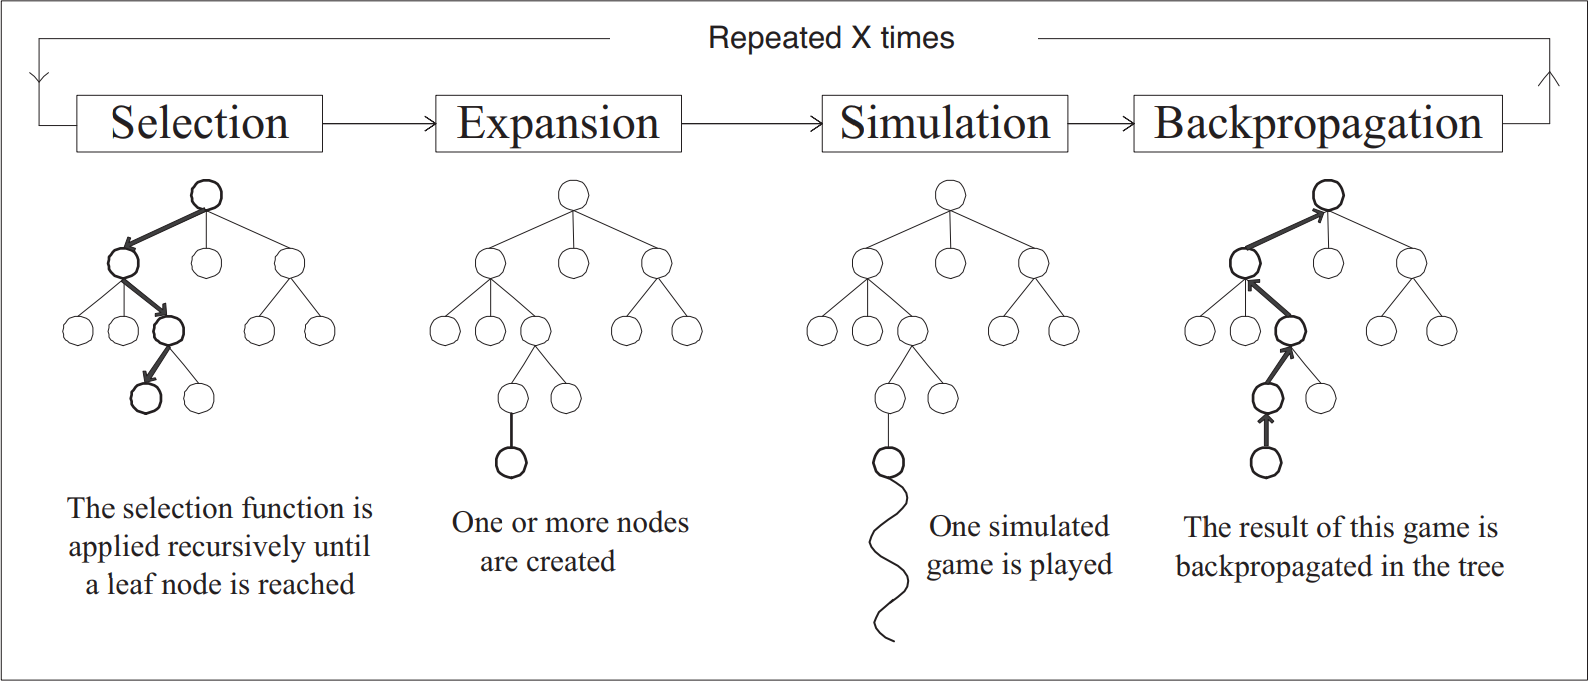
\includegraphics[width=0.5\textwidth]{MCTSProcess}
		    \caption{Overview of Monte-Carlo Tree Search. Image sourced from \cite{chaslot2008monte}. }
		    \label{fig:MCTS1}
		\end{figure}
		
		% Explination of MCTS stages
		The MCTS process is done in several stages, firstly a tree is built in an asymmetric and incremental way. Then for each iteration of the algorithm, a tree policy is used to fine the most urgent node of the current tree. The tree policy will then attempt to look in areas that have not been well sampled yet and areas which appear to be promising. A simulation is then run from the selected node and the tree is updated according to the result.

		
		MCTS is one of the most promising baseline approaches in the  literature.
		There has been a good deal of research on MCTS variants, each providing better results according to different domains \cite{browne2012survey, park2015mcts, perez2014knowledge, ilhan2017monte, de2016monte, frydenberg2015investigating}.


		\subsubsection{Evolutionary Algorithms} \label{sssec:num2}

		
		
		Alpha beta pruning
		
		minimax
		
		\subsubsection{Breadth First Search (BFS) }\label{sssec:BFS}
		This paper proposes an efficient implementation of BFS for GVGP \cite{EfficientBFS} uses a hash function.
		
		\subsubsection{Depth First Search}

		Depth First search with alpha-beta pruning \cite{knuth1975analysis} has achived superhuman performace in chess, checkers and orthello. However it has not been effective in Go \cite{silver2016mastering}.
		
		
		OLETS
		
		
		Evolutionary Algorithms
		(RHEA)
		
		
	
\section{Methodologies}	
		
		


\section{Conclusion}
The conclusion goes here.

% references section

\bibliographystyle{IEEEtran}
\bibliography{references}

% Appendices

\appendices
\section{First appendix}
Appendices are optional. Delete or comment out this part if you do not need them.

% that's all folks
\end{document}
